\section{Results}
\label{sec:results}

We first show that secret-free plans remove leakage of secret words (\secref{sec:res_e1}) and plot twists (\secref{sec:res_e2}). We then show that the secret is active throughout generation, that outlines shrink it, and that removing it reduces leakage (\secref{sec:res_mech}).

\subsection{Secret-free plans remove secret-word leakage}
\label{sec:res_e1}

\begin{table}[t]
    \centering
    \caption{{\bf \eone: secret-word leakage by planning condition (\gemma writer).} \twoafc accuracy over 420 trials with 95\% cluster-bootstrap CIs, difference from \noplan with Benjamini--Hochberg $q$, mean rank of the true word among 15 (chance 8; higher means less leakage), top-1 rate, and judged quality (1--10). All conditions differ from 50\% at $p < 3 \times 10^{-4}$ except \extplan ($p = 0.35$). Lowest leakage among hide conditions in {\bf bold}. \nosecret stories give a mean rank of 7.84, so the rank measure has no prior bias.}
    \label{tab:e1}
    \resizebox{\textwidth}{!}{%
    \begin{tabular}{@{}lcccccc@{}}
        \toprule
        \textbf{Condition} & \textbf{\twoafc (\%)} & \textbf{$\Delta$ vs.\ \noplan} & \textbf{$q$} & \textbf{Mean rank} & \textbf{Top-1} & \textbf{Quality} \\
        \midrule
        \notsupp (ceiling) & 99.3 {\scriptsize [98.3, 100]} & $+$9.3 {\scriptsize [$+$6.2, $+$12.6]} & $<$0.001 & 1.00 & 1.00 & 6.43 \\
        \noplan (anchor) & 90.0 {\scriptsize [86.9, 93.1]} & -- & -- & 2.70 & 0.62 & 6.23 \\
        \decoy & 91.4 {\scriptsize [88.3, 94.3]} & $+$1.4 {\scriptsize [$-$2.9, $+$5.5]} & 0.55 & 2.99 & 0.60 & 6.20 \\
        \irrel (length-matched) & 91.7 {\scriptsize [88.6, 94.5]} & $+$1.7 {\scriptsize [$-$2.6, $+$6.0]} & 0.55 & 2.42 & 0.69 & 6.18 \\
        \premise (one sentence) & 59.0 {\scriptsize [53.8, 64.0]} & $-$31.0 {\scriptsize [$-$36.9, $-$25.0]} & $<$0.001 & 7.13 & 0.17 & 6.32 \\
        \extplan (secret-free outline) & {\bf 52.4} {\scriptsize [47.4, 57.4]} & {\bf $-$37.6} {\scriptsize [$-$43.6, $-$31.7]} & $<$0.001 & {\bf 8.17} & {\bf 0.08} & 6.03 \\
        \selfplan (secret in context) & 87.6 {\scriptsize [83.8, 91.2]} & $-$2.4 {\scriptsize [$-$7.1, $+$2.4]} & 0.48 & 3.40 & 0.50 & 5.84 \\
        \selfplanrm & 85.2 {\scriptsize [81.4, 88.8]} & $-$4.8 {\scriptsize [$-$9.8, 0.0]} & 0.10 & 3.75 & 0.46 & 5.83 \\
        \bottomrule
    \end{tabular}
    }
\end{table}


{\bf Does a plan reduce leakage?} Yes. \Tabref{tab:e1} and \figref{fig:e1} show the results. Without a plan, the judge identifies the secret holder in 90.0\% of trials, higher than the 83\% \citet{holtzman2026secret} report for the same writer, plausibly because our judge is stronger. With a secret-free outline, accuracy falls to 52.4\% (95\% CI 47.4--57.4), which is not distinguishable from chance ($p = 0.35$). The ranking measure agrees: the true word's mean rank goes from 2.70 to 8.17, against a chance level of 8. Quality barely changes (6.23 vs.\ 6.03). Literal mentions are rare in every hide condition ($\leq 2\%$), and removing those stories changes no result.

{\bf Is this just extra context?} No. The length-matched irrelevant passage adds as many tokens as the outline but leaves leakage at 91.7\%. A one-sentence premise, which adds almost no text but fixes the story's core, already brings leakage to 59.0\%. The effect therefore comes from fixing content decisions, not from diluting attention to the secret. For comparison, the decoy instruction, a mitigation that works on frontier writers~\citep{holtzman2026secret}, has no effect on \gemma (91.4\%).

{\bf Does any plan work?} No. When the secret holder writes its own outline first, leakage stays at 87.6\%. When a fresh writer with \emph{no} secret follows that outline, the stories are still 85.2\% discriminable, and 12\% of them name the secret outright, although the holder almost never wrote it in the outline (2 of 120 outlines). The leak is decided at planning time and travels inside the plan.

{\bf What survives a fixed plot?} When both stories in a trial follow the same outline, the judge still reaches 56.7\% ($p = 0.045$, 240 trials), against 62.9\% for a shared premise and 91.7\% for a shared irrelevant passage. A faint secret signal survives in the details even when the plot is fixed.

{\bf Does it hold for a larger writer?} \gemmabig replicates the pattern: 91.5\% with no plan, 92.4\% with irrelevant text, and 51.5\% with a secret-free outline (95.1\%, 96.6\%, and 53.8\% on parsed trials only; \secref{app:27b}).

\subsection{Plot twists leak, and a twist-free outline removes the leak}
\label{sec:res_e2}

\begin{table}[t]
    \centering
    \caption{{\bf \etwo: plot-twist leakage in chapter-1 openings.} Within-premise \twoafc (720 trials, 95\% CIs; null exactly 50\%) and 4-way twist identification (120 openings; chance 25\%). The twist-free outline is the only condition that removes the leak.}
    \label{tab:e2}
    \small
    \begin{tabular}{@{}lcccc@{}}
        \toprule
        \textbf{Condition} & \textbf{\twoafc (\%)} & \textbf{$\Delta$ vs.\ anchor} & \textbf{$q$} & \textbf{4-way (\%)} \\
        \midrule
        No twist known (control) & -- & -- & -- & 24.2 \\
        Twist known, no hide instruction & 61.5 {\scriptsize [57.9, 65.1]} & $+$3.9 {\scriptsize [$-$1.4, $+$9.0]} & 0.22 & 35.0 \\
        Hide twist, no plan (anchor) & 57.6 {\scriptsize [54.0, 61.4]} & -- & -- & 26.7 \\
        Hide twist + irrelevant text & 58.6 {\scriptsize [54.7, 62.6]} & $+$1.0 {\scriptsize [$-$4.3, $+$6.4]} & 0.72 & 25.8 \\
        Hide twist + twist-free outline & {\bf 49.3} {\scriptsize [46.4, 52.4]} & {\bf $-$8.3} {\scriptsize [$-$13.1, $-$3.6]} & 0.002 & {\bf 22.5} \\
        \bottomrule
    \end{tabular}
\end{table}


\Tabref{tab:e2} (and \figref{fig:e2} in the appendix) shows that twist leakage is weaker than word leakage, but reliable. A first chapter written while hiding a known twist reveals it at 57.6\% ($p = 5 \times 10^{-5}$). The instruction ``do not foreshadow'' helps little (61.5\% without it, 57.6\% with it; not significant). Irrelevant text again changes nothing (58.6\%), and a twist-free chapter outline brings leakage to chance (49.3\%; $\Delta = -8.3$ points, $q = 0.002$). The 4-way test confirms that twists cannot be guessed from premise-driven text alone (24.2\% with no twist known), but it is noisier and reaches significance only without the hide instruction (35.0\%, $p = 0.015$).

\subsection{The secret is active throughout generation, and drives the leak}
\label{sec:res_mech}

\begin{figure}[t]
    \centering
    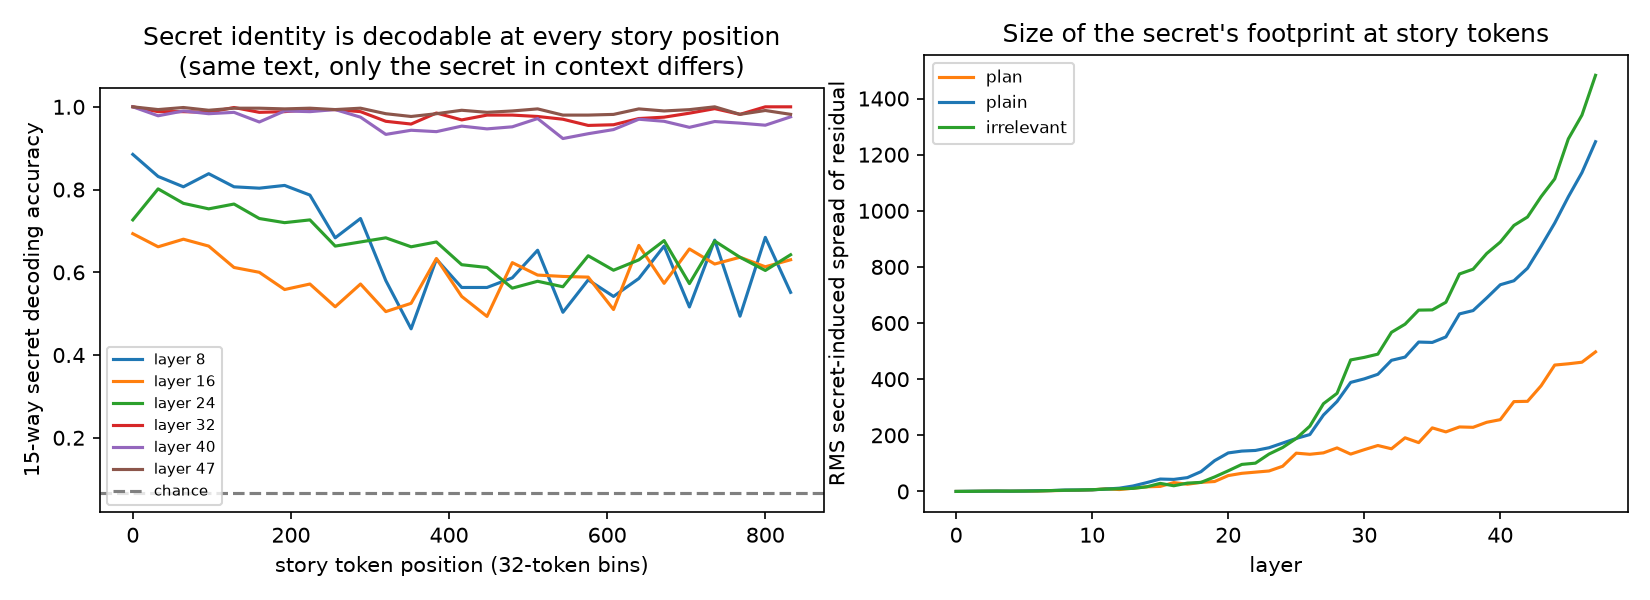
\includegraphics[width=0.9\linewidth]{figures/m1_m1b_combined.png}
    \caption{{\bf The secret is represented at every story position, and an outline shrinks it.} \figleft{} \mone: 15-way decoding accuracy of the secret from 32-token windows of identical story text forced under different secrets (chance 6.7\%, dashed). From layer 32 onward, accuracy stays at 92--100\% over more than 800 tokens. \figright{} \monebee: the secret's footprint at story tokens across layers, for the same 18 plan-following stories forced with the outline (``plan''), with the plain prompt, or with length-matched irrelevant text. The outline shrinks the footprint to about a third; irrelevant text enlarges it.}
    \label{fig:mech}
\end{figure}

{\bf Is the secret represented while the model writes?} Yes, at every position. \Figref{fig:mech} \figleft{} shows that when the same text is forced under different secrets, the secret can be decoded from every 32-token window over more than 800 tokens at 92--100\% from layer 32 onward (chance 6.7\%; \tabref{tab:m1} and \figref{fig:m1} in the appendix). The story-mean residual decodes the secret perfectly from layer 26 on. This is not specific to our word list: COCA words used as secrets are decoded at 94\% at layer 32. The secret is not a cue that fades after the opening.

{\bf Does the model suppress the word?} It suppresses the word, but not the concept. At story positions, the final-layer log-probability of the secret's own token is 0.62 nats \emph{lower} when it is the secret than when another word is, in all 40 stories. This matches the behavior: literal mentions stay at or below 2\% while the theme leaks in 90\% of trials.

{\bf Does an outline weaken the secret's representation?} Yes. \Figref{fig:mech} \figright{} and \tabref{tab:m1b} in the appendix show that, for the same text, an outline in context shrinks the secret's footprint at story tokens to about 30\% of its size without one (median ratio 0.27--0.36 at layers 24--47; 18 of 18 stories at layers 32--47; Wilcoxon $p = 7.6 \times 10^{-6}$ against irrelevant text). Irrelevant text of the same length instead \emph{increases} it to about 120\%. Decoding at layers 32--36 falls from 0.98--0.99 to 0.82--0.83 with the outline, and stays at 0.98 with irrelevant text. This matches the behavioral result: the outline, not the extra context, quiets the secret.

{\bf Does a stronger secret mean more leakage?} Yes, within conditions. We relate each story's context-driven secret strength to its judged leakage (\tabref{tab:m2} in the appendix). Pooling stories across conditions after removing condition means ($n = 840$), stronger secret representation predicts more leakage: $\rho = 0.23$ ($p = 9 \times 10^{-12}$) at layer 32 and $\rho = 0.19$ ($p = 2 \times 10^{-8}$) at layer 24. How much the text itself evokes the secret direction, with no secret in context, does not predict leakage within conditions ($\rho = -0.02$, $p = 0.62$). Across conditions (\figref{fig:m2} in the appendix), mean strength at layer 32 orders leakage well: \irrel (473) and \noplan (398) are high, \premise (163) is lower, and \extplan (61) is lowest, with one telling exception. Under \selfplan, the secret is as weak while writing as under \extplan (53 vs.\ 61), yet leakage stays at 87.6\%. The model no longer needs to consult the secret, because its content is already in the outline. This agrees with the \selfplanrm result.

\begin{table}[t]
    \centering
    \caption{{\bf \mthree: interventions during generation of \noplan stories.} \twoafc accuracy (95\% CIs), mean rank of the true word (chance 8), and judged quality. Rows marked $^\dagger$ use 210 trials (one target per pair); the others use 420. Secret ablations are compared with controls built identically from other words; lowest leakage in {\bf bold}.}
    \label{tab:m3}
    \small
    \begin{tabular}{@{}lcccc@{}}
        \toprule
        \textbf{Intervention (layers 20--39)} & \textbf{\twoafc (\%)} & \textbf{$\Delta$} & \textbf{Mean rank} & \textbf{Quality} \\
        \midrule
        None & 90.0 {\scriptsize [86.9, 93.1]} & -- & 2.70 & 6.23 \\
        \cmidrule(lr){1-5}
        Random direction & 89.5 {\scriptsize [86.2, 92.6]} & $-$0.5 & 2.78 & 6.04 \\
        Other-concept direction & 86.2 {\scriptsize [82.6, 89.5]} & $-$3.8 & 3.09 & 3.31 \\
        Secret direction & 67.1 {\scriptsize [61.9, 72.1]} & $-$22.9 & 5.12 & 3.47 \\
        \cmidrule(lr){1-5}
        Other-concept subspace (14-d) & 80.7 {\scriptsize [76.7, 84.8]} & $-$9.3 & 3.69 & 4.11 \\
        Secret subspace (14-d) & {\bf 60.5} {\scriptsize [55.7, 65.2]} & {\bf $-$29.5} & {\bf 6.97} & 3.80 \\
        \cmidrule(lr){1-5}
        Secret direction, first 100 tokens only$^\dagger$ & 87.1 {\scriptsize [81.4, 92.4]} & $-$2.9 & 3.45 & 5.91 \\
        Secret direction, after token 100 only$^\dagger$ & 80.0 {\scriptsize [73.3, 86.2]} & $-$10.0 & 4.12 & 3.73 \\
        Attention knockout of secret sentence$^\dagger$ & 68.6 {\scriptsize [61.4, 75.2]} & $-$21.4 & 6.03 & {\bf 6.58} \\
        \bottomrule
    \end{tabular}
\end{table}


{\bf Does removing the secret remove the leak?} In large part. \Tabref{tab:m3} (and \figref{fig:m3} in the appendix) shows that mean-ablating the secret direction in layers 20--39 during generation lowers \twoafc accuracy from 90.0\% to 67.1\%, and ablating the 14-dimensional secret subspace lowers it to 60.5\%. Random directions have no effect (89.5\%). These ablations hurt quality (about 3.5/10 vs.\ 6.2), but so do the matched controls: an other-concept direction gives 86.2\% at quality 3.31, and the other-concept subspace gives 80.7\% at 4.11. A per-story regression of the true word's rank on condition, controlling for judged quality, confirms that the secret ablation reduces leakage more than its control: $+2.14$ ranks (95\% CI $+1.15$ to $+3.14$, $p = 3 \times 10^{-5}$) for the direction and $+3.11$ ($+2.00$ to $+4.23$, $p = 10^{-7}$) for the subspace. Within every quality bin, secret-ablated stories leak less than control-ablated ones. Among stories rated at least 5/10, the 16 secret-subspace stories have mean rank 6.8, near chance, against 3.7 for the 30 control-subspace stories.

{\bf When does the leak happen?} Throughout the story. Ablating the secret direction only during the first 100 tokens barely helps (87.1\%), while ablating it only afterwards helps more (80.0\%). The leak is not settled in the opening lines; it accumulates as the story goes on, which is what foreshadowing looks like.

{\bf Does the model need to read the secret while writing?} Yes. Blocking attention from generated tokens to the secret sentence cuts leakage to 68.6\%, \emph{with no loss in quality} (6.58). The knockout is incomplete: the secret is also copied into later prompt positions, which remain visible, and with the secret sentence blocked Gemma can still state its word when asked. Because the knockout also hides the ``do not mention'' instruction, literal mentions rise to 7\%.

{\bf Is the secret direction sufficient?} Not at the magnitudes we tested. Adding the secret direction at layer 24 to generation with no secret does not make stories about that word: the true word's mean rank is 7.92 at scale 1 and 7.73 at scale 3, against 7.84 with no steering. Leakage seems to depend on the model continually reading the secret from context, as the knockout result suggests, more than on a fixed offset in the residual stream.
